\section{Instalación del servidor principal de FreeIPA}\label{sec:instalacion-servidor-principal}

Inicialmente, se llevó a cabo la creación de la máquina virtual destinada a alojar el servidor principal de la infraestructura. Sobre esta se instaló el sistema operativo Fedora Server 44, seleccionado de acuerdo con los requisitos y las recomendaciones de compatibilidad establecidas para la implementación de la plataforma FreeIPA. Asimismo, la máquina virtual se configuró de acuerdo con las especificaciones técnicas definidas durante la fase de diseño, considerando los recursos de procesamiento, memoria, almacenamiento y conectividad necesarios para el correcto funcionamiento del servicio implementado, como se muestra en la \autoref{fig:creacion-vm-ipa1}.

\begin{figure}[H]
	\centering
	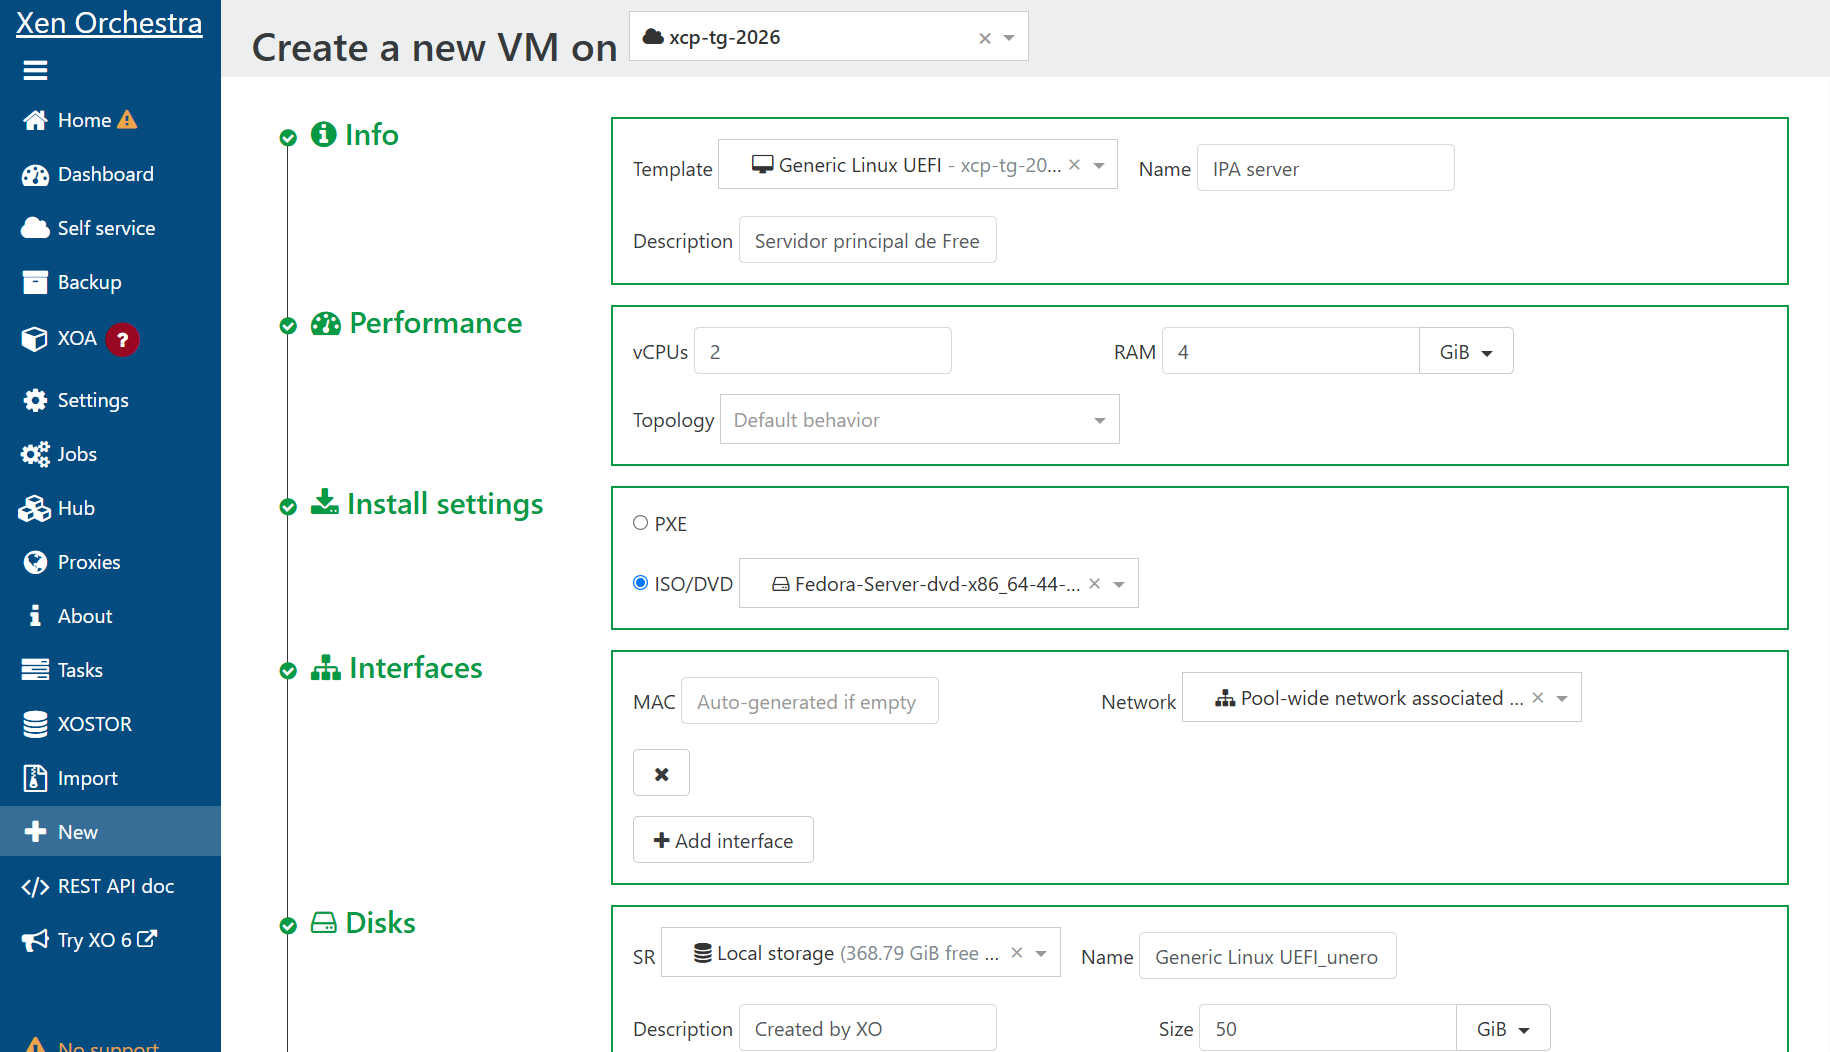
\includegraphics[width=0.9\textwidth]{mainmatter/II-desarrollo-metodologico/implementacion/imagenes/creacion-vm-ipa1.png}
	\caption{Creación de la máquina virtual del servidor principal}
	\label{fig:creacion-vm-ipa1}
\end{figure}

Posteriormente, se realizó la instalación del sistema operativo sobre la máquina virtual creada previamente, como se muestra en la \autoref{fig:instalacion-sistema-operativo}.

\begin{figure}[H]
	\centering
	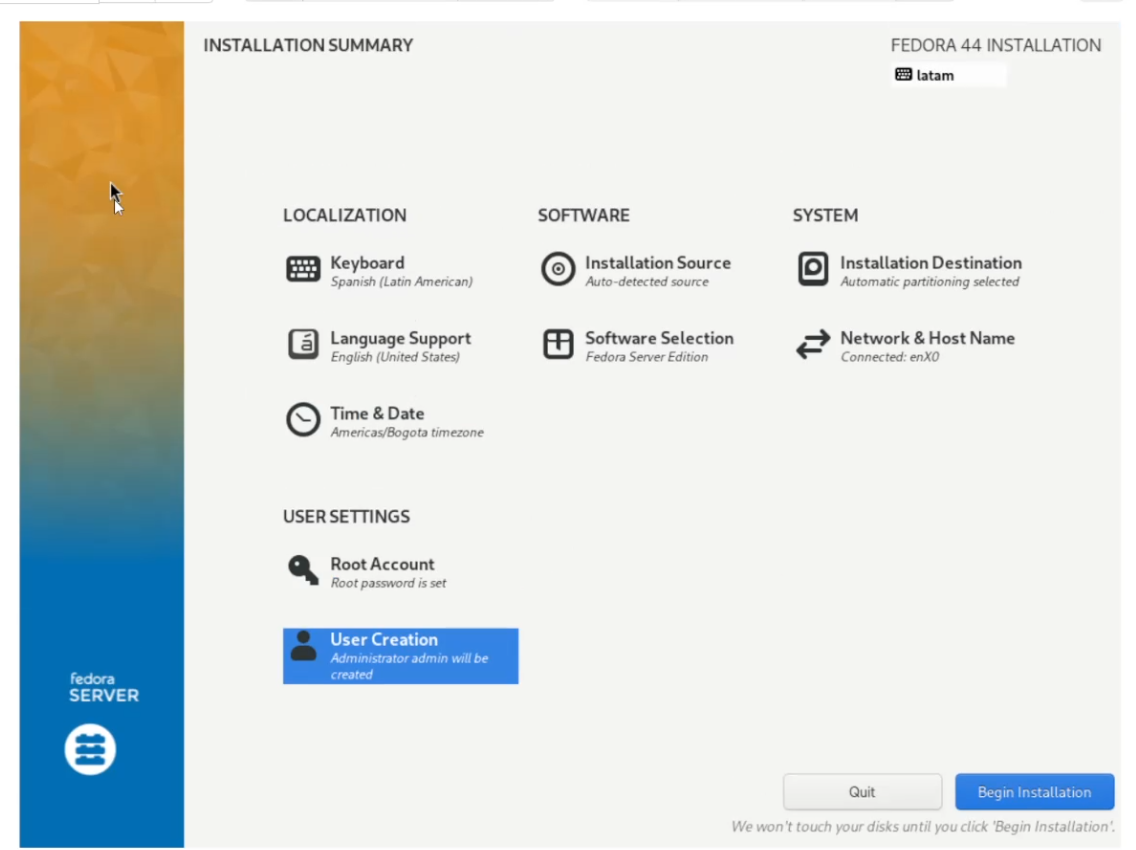
\includegraphics[width=0.9\textwidth]{mainmatter/II-desarrollo-metodologico/implementacion/imagenes/instalacion-sistema-operativo.png}
	\caption{Instalación del sistema operativo Fedora Server 44 en el servidor principal}
	\label{fig:instalacion-sistema-operativo}
\end{figure}

Como parte de la configuración inicial del sistema, se configuró la interfaz de red de la máquina virtual, asignándole la dirección \acs{IP} previamente definida dentro del esquema de direccionamiento de la infraestructura. Esta configuración garantiza la conectividad con los demás componentes del entorno y constituye un requisito indispensable para la instalación y configuración del servidor FreeIPA. En la \autoref{fig:configuracion-ip-ipa1} se observa la configuración de red realizada.

\begin{figure}[H]
	\centering
	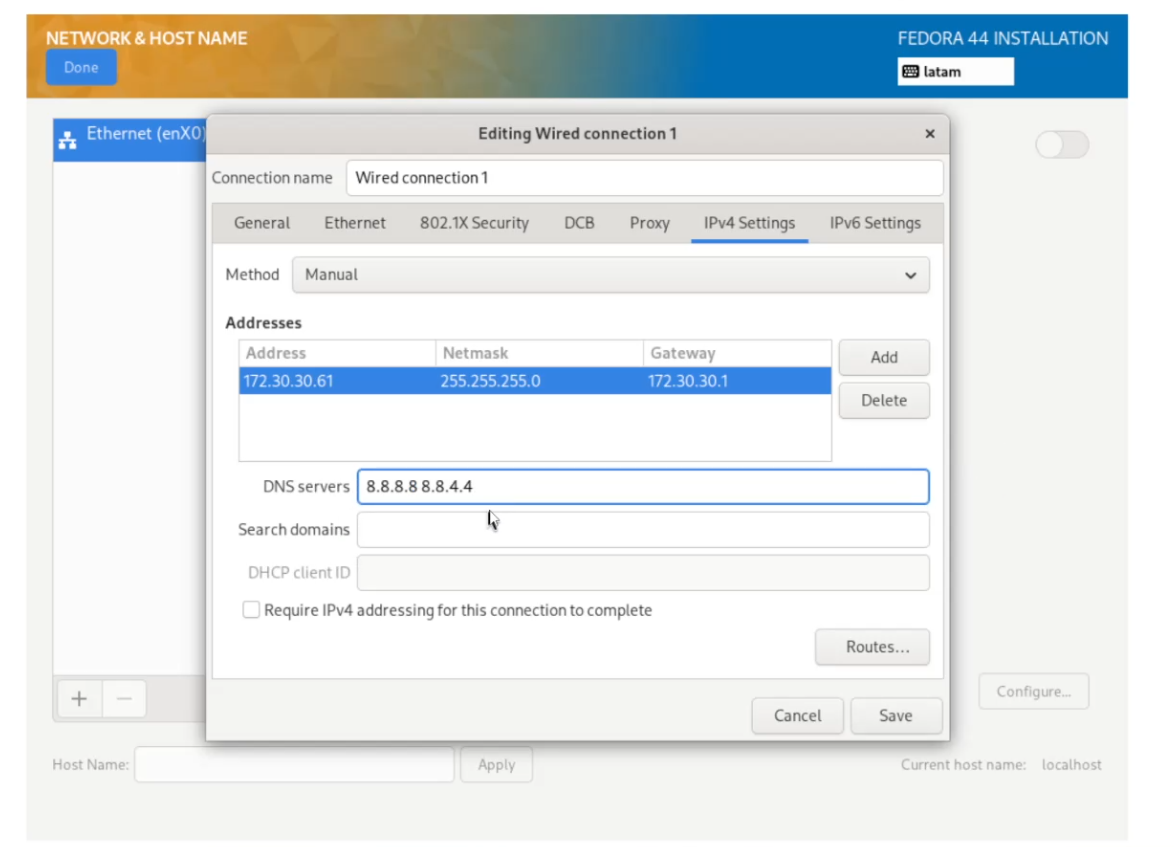
\includegraphics[width=0.9\textwidth]{mainmatter/II-desarrollo-metodologico/implementacion/imagenes/configuracion-ip-ipa1.png}
	\caption{Configuración de la interfaz de red de la máquina virtual}
	\label{fig:configuracion-ip-ipa1}
\end{figure}

Una vez finalizada la instalación del sistema operativo, se realizaron las configuraciones previas requeridas para la instalación de FreeIPA, siguiendo el procedimiento recomendado en la documentación oficial del proyecto. Como primer paso, se configuró el nombre de dominio completamente calificado (\acs{FQDN}) del servidor, utilizando el nombre \textbf{ipa1.grid.uniquindio.edu.co}, como se muestra en la \autoref{fig:nombre-host-ipa1}.

\begin{figure}[H]
	\centering
	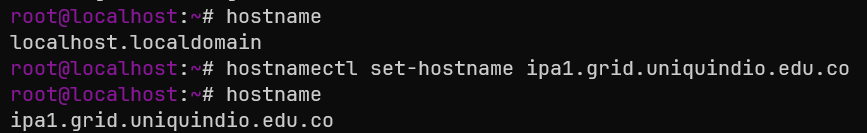
\includegraphics[width=0.9\textwidth]{mainmatter/II-desarrollo-metodologico/implementacion/imagenes/nombre-host-ipa1.png}
	\caption[Configuración del nombre de dominio]{Configuración del nombre de dominio completamente calificado del servidor principal de FreeIPA}
	\label{fig:nombre-host-ipa1}
\end{figure}

Posteriormente, se agregó la entrada correspondiente al servidor en el archivo \path{/etc/hosts}, asociando la dirección \acs{IP} \textbf{172.30.30.61} con el nombre de dominio \textbf{\nolinkurl{ipa.grid.uniquindio.edu.co}} y su nombre corto \textbf{ipa1}. Esta configuración permite la correcta resolución local del nombre del servidor, requisito necesario para el adecuado funcionamiento y la instalación de FreeIPA. El resultado de esta modificación se ilustra en la \autoref{fig:archivo-hosts-ipa1}.

\begin{figure}[H]
	\centering
	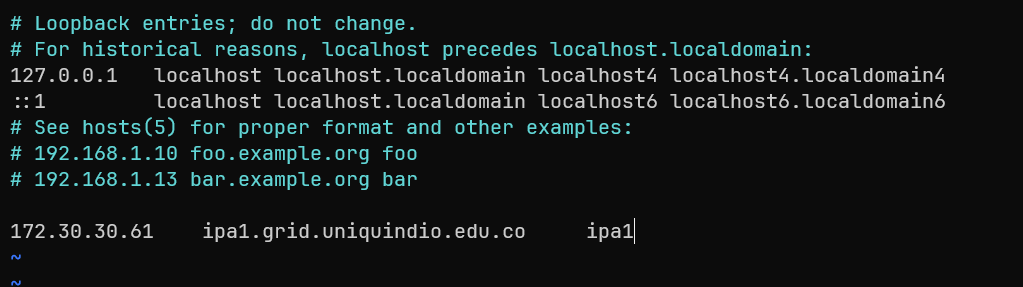
\includegraphics[width=0.9\textwidth]{mainmatter/II-desarrollo-metodologico/implementacion/imagenes/archivo-hosts-ipa1.png}
	\caption{Configuración del archivo /etc/hosts}
	\label{fig:archivo-hosts-ipa1}
\end{figure}

Posteriormente, se configuraron las reglas del cortafuegos necesarias para el funcionamiento del servidor FreeIPA. Para ello, se habilitaron de forma permanente los servicios correspondientes a \ac{LDAP} y \ac{LDAPS} y, a continuación, se recargó la configuración del cortafuegos con el fin de aplicar los cambios realizados.

Esta configuración permite que los diferentes componentes de la infraestructura puedan establecer comunicación con el servidor y garantiza la disponibilidad de los servicios requeridos para los procesos de autenticación y administración centralizada. En la \autoref{fig:reglas-cortafuegos-ipa1} se presenta el procedimiento realizado y el resultado obtenido tras la verificación de la configuración.

\begin{figure}[H]
	\centering
	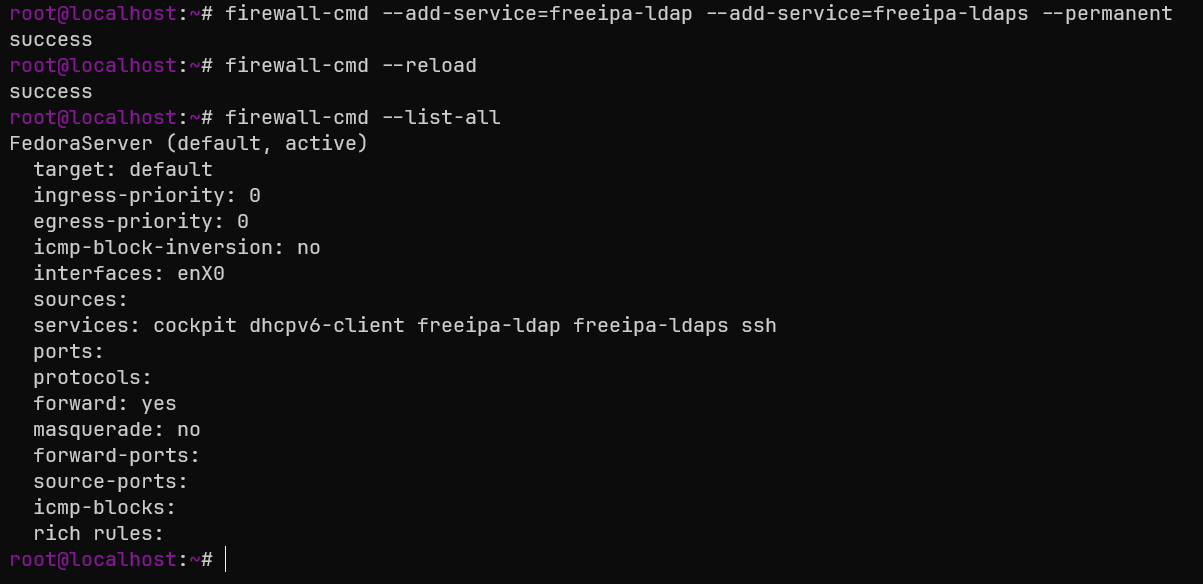
\includegraphics[width=0.9\textwidth]{mainmatter/II-desarrollo-metodologico/implementacion/imagenes/reglas-cortafuegos-ipa1.png}
	\caption{Configuración de las reglas del cortafuegos para los servicios de FreeIPA}
	\label{fig:reglas-cortafuegos-ipa1}
\end{figure}

Una vez completadas las configuraciones previas del sistema, se procedió a la instalación del paquete freeipa-server mediante el gestor de paquetes dnf, el cual contiene los componentes necesarios para el despliegue y la administración del servidor FreeIPA. En la \autoref{fig:instalacion-paquete-ipa1} se observa la ejecución de este procedimiento.

\begin{figure}[H]
	\centering
	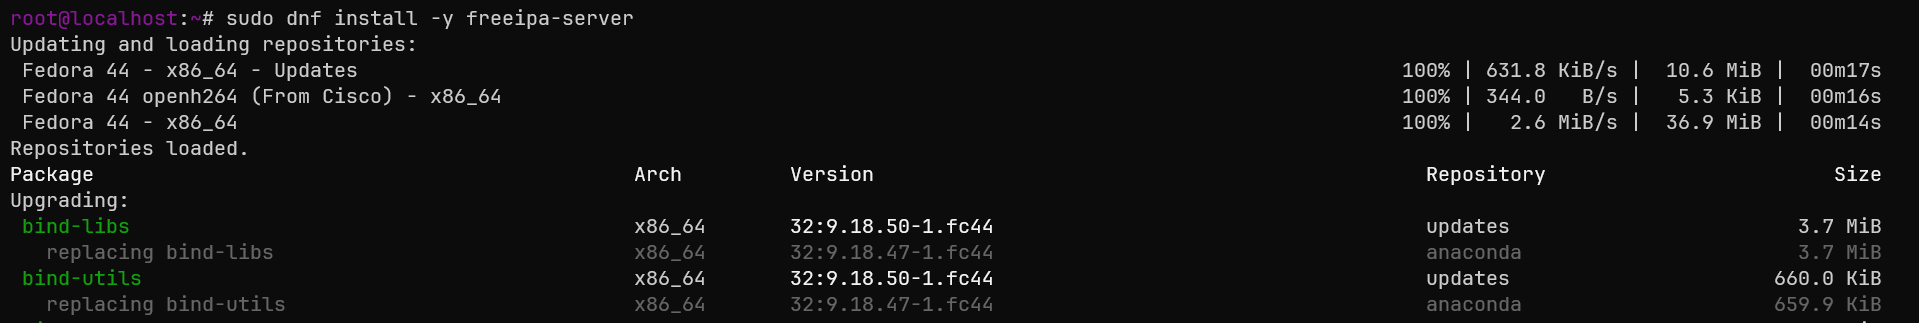
\includegraphics[width=0.8\textwidth]{mainmatter/II-desarrollo-metodologico/implementacion/imagenes/instalacion-paquete-ipa1.png}
	\caption{Instalación del paquete freeipa-server}
	\label{fig:instalacion-paquete-ipa1}
\end{figure}

Posteriormente, se ejecutó el comando ipa-server-install, el cual inicia el proceso de instalación y configuración de FreeIPA a través de un asistente interactivo. Debido a que el nombre de dominio completamente calificado (\ac{FQDN}) ya había sido definido previamente como ipa1.grid.uniquindio.edu.co, el instalador detectó automáticamente parte de la información requerida y propuso los valores predeterminados correspondientes.

Entre los parámetros configurados se encuentra el \ac{FQDN} \nolinkurl{ipa1.grid.uniquindio.edu.co}, utilizado para identificar de manera única el servidor dentro de la infraestructura. A partir de este valor se determinó el dominio grid.uniquindio.edu.co, mientras que el dominio de Kerberos (realm) se estableció como \nolinkurl{GRID.UNIQUINDIO.EDU.CO}, siguiendo la convención de utilizar letras mayúsculas para este tipo de identificadores.

Asimismo, se definieron las credenciales correspondientes al usuario Directory Manager, encargado de las tareas administrativas del servicio de directorios, y al usuario admin, utilizado para la administración de la plataforma FreeIPA. Del mismo modo, se configuró el nombre de NetBIOS \ac{GRID}, necesario para garantizar la compatibilidad con determinados servicios y mecanismos de interoperabilidad.

Por otra parte, el instalador detectó la dirección \acs{IP} 172.30.30.61, correspondiente al servidor principal, la cual fue utilizada como base para la configuración de red del servicio.

Finalmente, el asistente llevó a cabo la instalación y configuración de los distintos componentes de la plataforma, entre los que se encuentran 389 Directory Server, el Centro de Distribución de Claves de Kerberos (\acs{KDC}), la autoridad certificadora (\acs{CA}), el servidor web Apache y los servicios encargados de la gestión centralizada de identidades y certificados. Las \autoref{fig:instalacion-servidor-ipa1-paso-1} y \autoref{fig:instalacion-servidor-ipa1-paso-2} presentan el procedimiento de instalación y los parámetros definidos durante este proceso.

\begin{figure}[H]
	\centering
	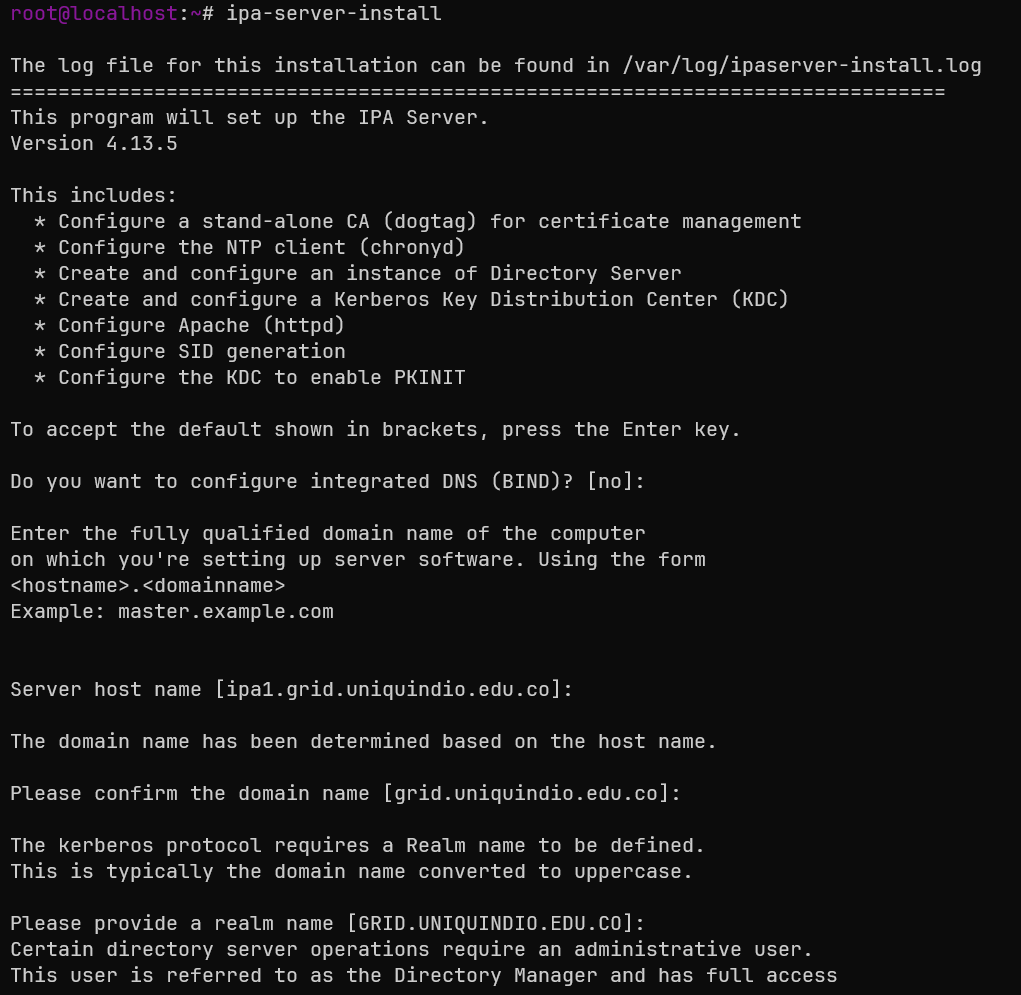
\includegraphics[width=0.6\textwidth]{mainmatter/II-desarrollo-metodologico/implementacion/imagenes/instalacion-servidor-ipa1-paso-1.png}
	\caption{Proceso de instalación y configuración inicial de FreeIPA parte 1}
	\label{fig:instalacion-servidor-ipa1-paso-1}
\end{figure}

\begin{figure}[H]
	\centering
	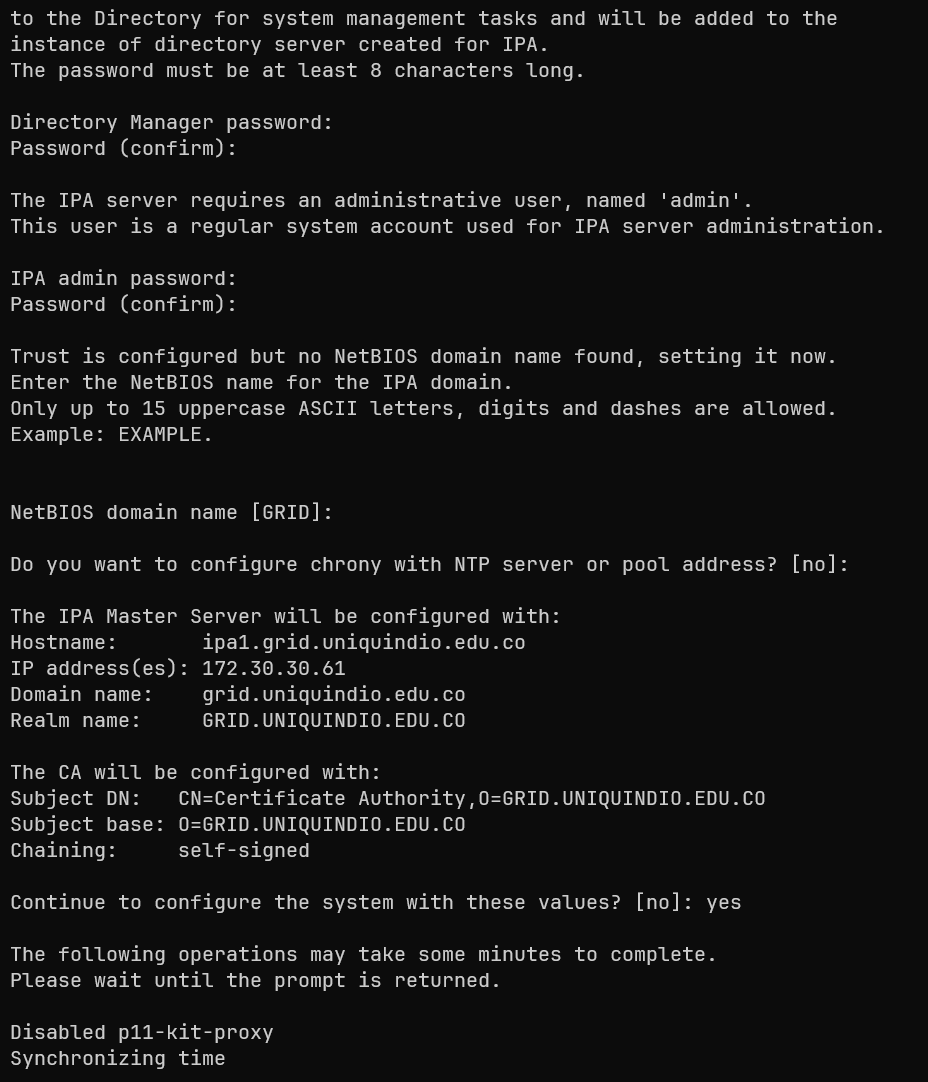
\includegraphics[width=0.6\textwidth]{mainmatter/II-desarrollo-metodologico/implementacion/imagenes/instalacion-servidor-ipa1-paso-2.png}
	\caption{Proceso de instalación y configuración inicial de FreeIPA parte 2}
	\label{fig:instalacion-servidor-ipa1-paso-2}
\end{figure}
